\documentclass{article}

\usepackage{booktabs}
\usepackage{tabularx}
\usepackage{graphicx}
\usepackage{color}
\usepackage{float}
\usepackage[colorlinks=true,urlcolor=blue]{hyperref}

\title{SE 3XA3: Development Plan\\Mari0}

\author{Team 9, Ninetendo
		\\ David Hobson hobsondd
		\\ Jose Miguel Ballesteros ballesjm
		\\ Jeff Pineda pinedaj
}

\date{}

%% Comments

\usepackage{color}

\newif\ifcomments\commentstrue

\ifcomments
\newcommand{\authornote}[3]{\textcolor{#1}{[#3 ---#2]}}
\newcommand{\todo}[1]{\textcolor{red}{[TODO: #1]}}
\else
\newcommand{\authornote}[3]{}
\newcommand{\todo}[1]{}
\fi

\newcommand{\wss}[1]{\authornote{blue}{SS}{#1}}
\newcommand{\ds}[1]{\authornote{red}{DS}{#1}}
\newcommand{\mj}[1]{\authornote{red}{MSN}{#1}}
\newcommand{\cm}[1]{\authornote{red}{CM}{#1}}
\newcommand{\mh}[1]{\authornote{red}{MH}{#1}}

% team members should be added for each team, like the following
% all comments left by the TAs or the instructor should be addressed
% by a corresponding comment from the Team

\newcommand{\tm}[1]{\authornote{magenta}{Team}{#1}}


\begin{document}

\begin{table}[hp]
\caption{Revision History} \label{TblRevisionHistory}
\begin{tabularx}{\textwidth}{llX}
\toprule
\textbf{Date} & \textbf{Developer(s)} & \textbf{Change}\\
\midrule
2016-09-30 & Jose Ballesteros & Added Coding Style and created Gantt Chart to be pointed to\\
2016-09-30 & David Hobson & Added Team Meeting Plan, Team Communication Plan, Team Member Roles\\
2016-09-30 & Jeff Pineda & Added Git Workflow Plan, Proof of Concept Demonstration, Technology\\
2016-10-21 & Jeff Pineda & Modified Proof of Concept Demonstration secton to accurately represent what is/was demonstrated, and updated Technology section to include new IDE being used and the selection of a testing framework.\\
... & ... & ...\\
\bottomrule
\end{tabularx}
\end{table}

\newpage

\maketitle

\textcolor{red}{ Include this text in a section named Abstract - CM} \\
This program is a game that is similar to Mari0 and will be created in Unity. Mari0 is a crossover of Super Mario Bros. and Portal.

\section{Team Meeting Plan}
\textcolor{red}{Add details regarding roles during meetings, to what extent things are discussed and follow up plans - CM} \\
Our team will be meeting at the regular lab times to quickly discuss changes as well as upcoming deadlines for the project. Our lab times are Wednesday from 8:30 - 10:20 and Friday 2:30 - 4:20. The majority of each meeting will be focused on the closest deadline to be met, discussing each members' schedules and using that information to create a work plan to meet the next deliverable. The rest of the meeting time will be used to discuss changes/issues that need to be addressed in regards to previous delivarables, and to talk about future delivarabes. If there are other times that we need to meet, we will discuss using the Facebook chat to decide on a time where all team members are available. 

\section{Team Communication Plan}
The communication will mainly happen through a Facebook chat that all team members have access to. Everyone apart of the chat can communicate quickly and effectively about milestones, changes, and meetings. Any shared files will be pushed to the repository on GitLab that everyone in the group has access to. E-mail may be used as well to send certain files or messages but this will be used rarely. 

\section{Team Member Roles}
\textbf{Project Leader and Developer:}  David Hobson\\
\textbf{Developer and Graphic Designer:}  Jose Miguel Ballesteros\\
\textbf{Developer and Documentation Manager:}  Jeff Pineda\\

\section{Git Workflow Plan}
\textcolor{red}{Include education or workshops needed to reach the experience necessary for feature branch workflow - CM} \\
Since we all have limited experience with Git, we will be utilizing a centralized workflow in the early stages of the project. However, as we get more comfortable with Git and when the need for multiple people to work on one file at the same time becomes more frequent, we will move to a featured branch workflow.

\section{Proof of Concept Demonstration Plan}
\textcolor{red}{Include more specific requirements in last paragraph - CM} \\
The most difficult part of the implementation of Mari0 will be coding the 'portals' and their mechanics. Two portals can be placed anywhere within line of sight of the main character and on any surface. These two portals are connected, with any projectile or character entering through one portal exits out of the other portal, maintaining their physical properties, such as acceleration and velocity, they had when first entering.

Testing whether or not player inputs lead to correct gameplay/visual outputs will be relatively simple, as this can be handled by writing unit tests. Testing the other aspects of the game such as puzzle difficulty, control feel and responsiveness, and enjoyability of the game will be more difficult. Testing these will need to be done through beta tests and player survey feedback.

For the proof of concept demonstration, we will demonstrate a simple level design to show working character physics, working character animations, and most of the portal mechanics. The portal mechanics to be demonstrated are the property that two portals are connected, and the player will maintain the physical properties they had when entering the first portal upon exiting the second portal. The ability to place portals on any surface will not be implemented by the time of the proof of concept demonstration.

\section{Technology}
\textcolor{red}{Include details about documentation for your C\# code and look into using a testing framework to aid in assert methods, running synchronously and other helpful methods - CM} \\
We will be using the Unity game engine to handle game physics and will be writing the rest of the game with C\#.
Members of the group will either use MonoDevelop, a Unity integrated IDE, or Visual Studio for coding. and we will be writing our own unit tests. We will be using NUnit as our unit-testing framework.

\section{Coding Style}
We will be using \href{https://msdn.microsoft.com/en-us/library/ff926074.aspx}{Microsoft's coding convention for C\#} with a couple alterations.
\begin{itemize}

  \item Open curly braces will follow the expression?s parameters and the closing brace will be inline with the expression as shown in figure 1 below.

\begin{figure}[H]
\centering
  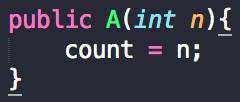
\includegraphics[width=30mm,scale = 0.25]{curlyBraces.jpg}
\end{figure}

  \item \textcolor{red}{Upper or Lower camel case? - CM} \\ All constants will be named in capital letters

  \item Method names will be named in camel case format.

\end{itemize}

\section{Project Schedule}
\textcolor{red}{Add run for any non-HTTP run protocols. Also, adjust task resources to below 100 percent  - CM} \\
\href{run:../../ProjectSchedule/ProjectSchedule.gan}{Click here for the Gantt Chart.}

\section{Project Review}

\end{document}